\documentclass[12pt]{article}

\usepackage[brazil]{babel}   
\usepackage[latin1]{inputenc}

\usepackage{sbc-template}

\usepackage{graphicx,url}


     
\sloppy

\title{Controle para basculante}

\author{Gilson da Rosa Webber\inst{1}, Rafael da Fonte Lopes da Silva\inst{1}}


\address{Instituto de Informática -- Universidade Federal do Rio Grande do Sul
  (UFRGS)\\
  Caixa Postal 15.064 -- 91.501-970 -- Porto Alegre -- RS -- Brazil
  \email{gilson.webber@inf.ufrgs.br, rflsilva@inf.ufrgs.br}
}

\begin{document} 

\maketitle


\section{Proposta geral}
Nossa proposta é a de construir um dispositivo microcontrolado com um \textbf{PIC-16F684} da $MicroChip^{TM}$ capaz de gerenciar a abertura de uma janela do tipo basculante, de acordo com o nível de luminosidade ambiente desejado pelo usuário. Desejamos projetá-lo de modo que opere de acordo com os seguintes possíveis critérios:

\begin{itemize}
\item Controle manual da abertura, feito pelo usuário;
\item Controle automático, definido de acordo com o grau de iluminação do ambiente onde estiver posicionado um sensor.
\end{itemize}

\subsection{Componentes}
\begin{figure}[ht]
\begin{center}
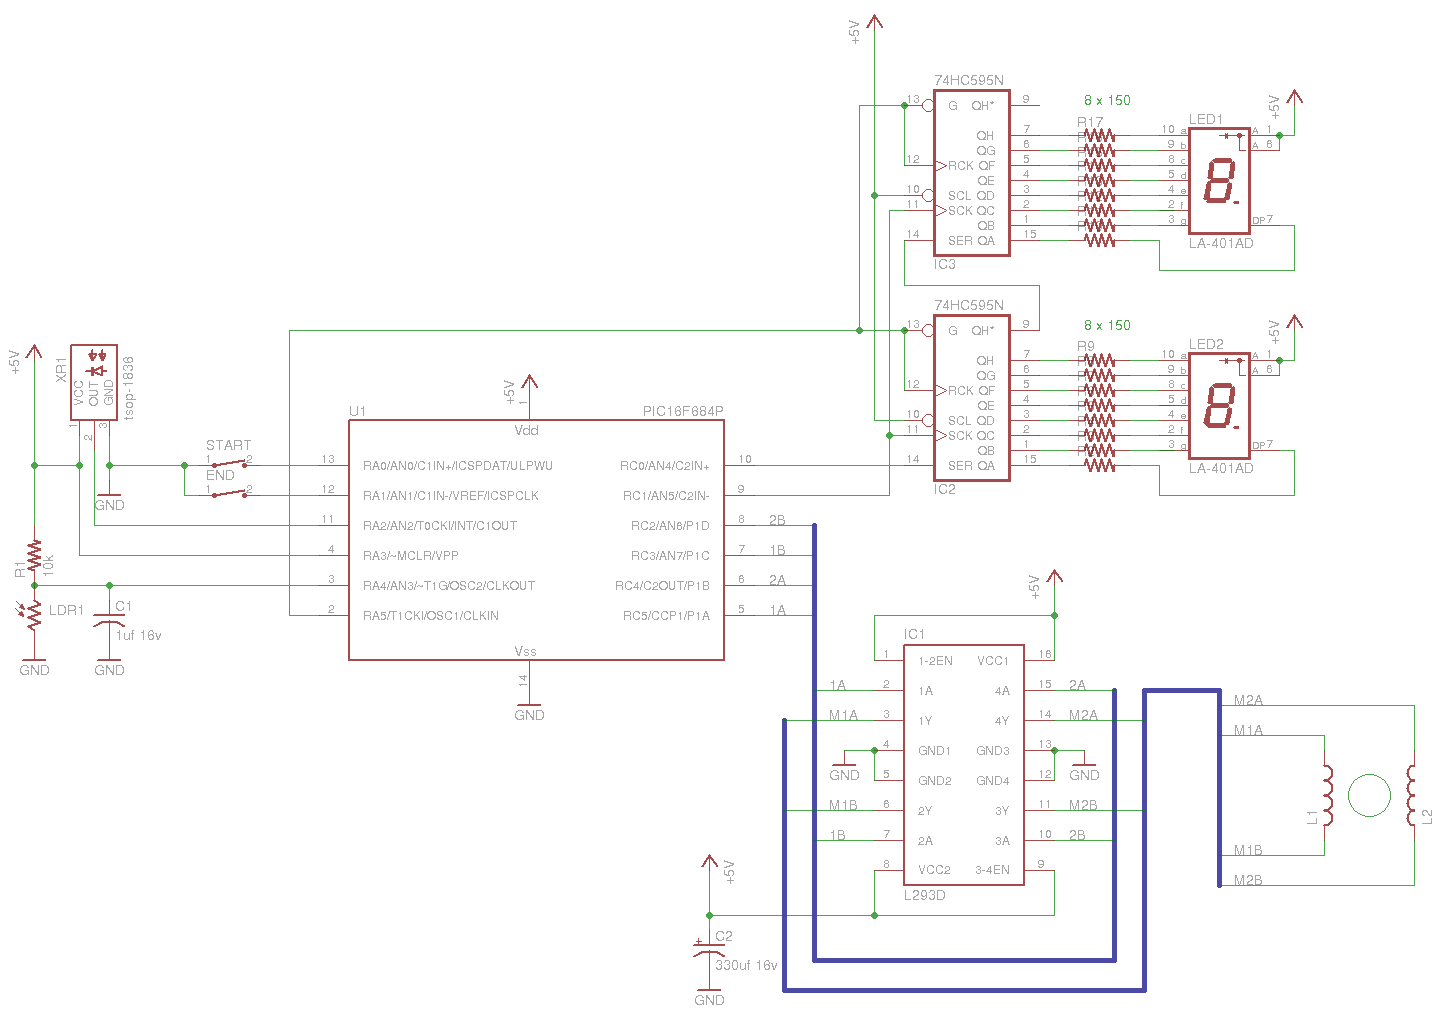
\includegraphics[scale=0.5]{Esquematico.png} 
\caption{Esquemático do projeto.}
\end{center}
\end{figure}

Para a implementação deste projeto, utilizaremos os seguintes componentes principais:

\begin{itemize}
\item Microcontrolador \textbf{PIC-16F684};
\item Um LDR;
\item Um receiver de infravermelho TSOP-1836;
\item Um IC Driver L293D;
\item Um motor de passo;
\item Dois IC Shifters 74HC595;
\item Dois displays de 7 segmentos LA-401AD.
\end{itemize}

\subsection{Funcionamento}
O funcionamento do projeto se dará da seguinte forma: o resistor LDR medirá a luminosidade do ambiente onde ele estiver inserido. Os valores de luminosidade serão lidos pelo conversor A/D do microcontrolador, o qual, quando estiver em modo automático, realizará os ajustes necessários para manter um certo nível de luminosidade, escolhido pelo usuário. Estes ajustes serão realizados pelo do motor de passo, que será controlado através da utilização do IC de driver do motor.

Quando em modo automático, o microcontrolador de tempos em tempos irá verificar o valor lido do LDR. Neste modo, ainda, o receiver de infravermelho pode gerar interrupções no microcontrolador quando o usuário quiser utilizar o controle remoto para acessar certas funcionalidades. Dentre as opções disponíveis, ele pode "setar" um valor de luminosidade a ser alcançado pelo dispositivo com alterações feitas pelo motor (de modo que a luminosidade ambiente se mantenha aproximadamente constante), ou então colocar o dispositivo em modo manual. Para realizar esta alteração com o controle, o usuário poderá utilizar o teclado numérico do controle.

Em modo manual, o usuário poderá ajustar a abertura da basculante com ação direta sobre o motor de passo, utilizando-se das teclas do controle remoto. Além disso, neste modo lhe será permitido visualizar o valor atual lido do LDR sobre a luminosidade.

Os valores de luminosidade, nos dois casos (manual e automático) poderão ser vistos pelo usuário com a ajuda dos dois displays de 7 segmentos ligados ao microcontrolador. Utilizaremos de forma serial os bits iniciais da porta C do PIC para isso (juntamente com os shifters).

\nocite{*}


\bibliographystyle{sbc}
\bibliography{report}

\end{document}
